% $Header: /cvsroot/latex-beamer/latex-beamer/solutions/conference-talks/conference-ornate-20min.en.tex,v 1.7 2007/01/28 20:48:23 tantau Exp $

\documentclass{beamer}
\setbeamertemplate{caption}[numbered]
\setbeamertemplate{footline}[frame number]
\setbeamerfont{caption}{size=\scriptsize}

\setbeamercolor{caption name}{fg=black}
\mode<presentation>
{
	\usetheme{default}
}


\usepackage[T2A]{fontenc} % Установка кодировки шрифта
\usepackage[utf8]{inputenc} % Установка кодировки исходного текста
\usepackage[english,russian]{babel} % Подключение локализации и переносов для русского и английского языков
\usepackage{amsmath,amssymb} % Подключение математических символов и формул
\usepackage{autonum} % Автоматическая нумерация формул только при наличии ссылок на них
\usepackage{wrapfig} % Подключение пакета для обтекания текстом рисунков и таблиц
\usepackage{array} % Подключение пакета для работы с таблицами
\usepackage{times}
% Or whatever. Note that the encoding and the font should match. If T1
% does not look nice, try deleting the line with the fontenc.
\usepackage{outlines}
\usepackage[T1]{fontenc}
\usepackage{graphicx}
\usepackage{caption}
\usepackage{subcaption}
\usepackage{colortbl} 




\title[] % (optional, use only with long paper titles)
{Разработка интеллктуальной системы анализа патентов химической отрасли\\ для представления данных в структурированном виде}

%\subtitle
%{Include Only If Paper Has a Subtitle}

\author[] % (optional, use only with lots of authors)
{\textbf{Студент 2-го курса:} Кайда Анатолий Сергеевич \\  
\textbf{Научный руководитель:} Глинский Андрей Владимирович}


\institute[]
{
	
}


\date[\today] 
{}


\subject{}
% latex or pdflatex,
% resp., then you can add a logo as follows:
 \pgfdeclareimage[height=0.9cm]{university-logo}{images/logo_mipt} \logo{\pgfuseimage{university-logo}}



\begin{document}
	
	\begin{frame}
		\titlepage
	\end{frame}
	
	
	\begin{frame}{Формулировка проблемы}
		% - A title should summarize the slide in an understandable fashion
		%   for anyone how does not follow everything on the slide itself.
		\begin{itemize}
			\item Количество ежегодно публикуемых статей и патентов в химии растет экспоненциально
			\item Процесс работы с в патентной и литературной информацией по-прежнему остается в значительной степени ручным
			\item Сложность навигации в большом объеме литературы приводит к тому, что важные научные открытия остаются незамеченными в течение длительного времени
		\end{itemize}
	
	\begin{figure}
		\centering
		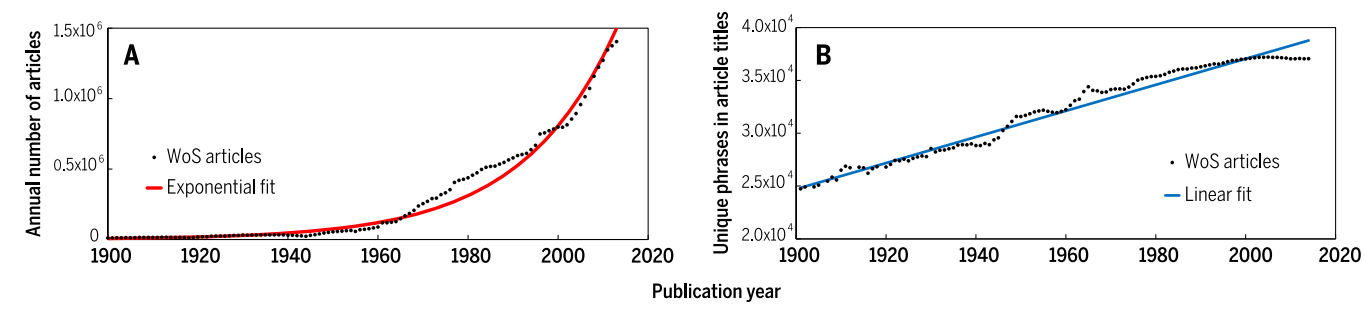
\includegraphics[width=1\textwidth]{images/growth_of_science.png}
		\caption[pt9]{(A) Годовой выпуск научных статей, индексированных в базе данных WoS. (B) Рост идей, охватываемых статьями, индексированными в WoS. Это было определено путем подсчета уникальных заглавных фраз (концепций) в фиксированном количестве статей.}
		\label{fig: growth_of_science}
	\end{figure}
			
				
						 
	
	\end{frame}
	
	\begin{frame}{Формулировка проблемы}
		{\scriptsize1. Ananikov V. Top 20 Influential AI-Based Technologies in Chemistry. Chemistry, 2024.}
		
		В последние годы набирает обороты <<цифровизация>> химии.
		\begin{figure}
			\centering
			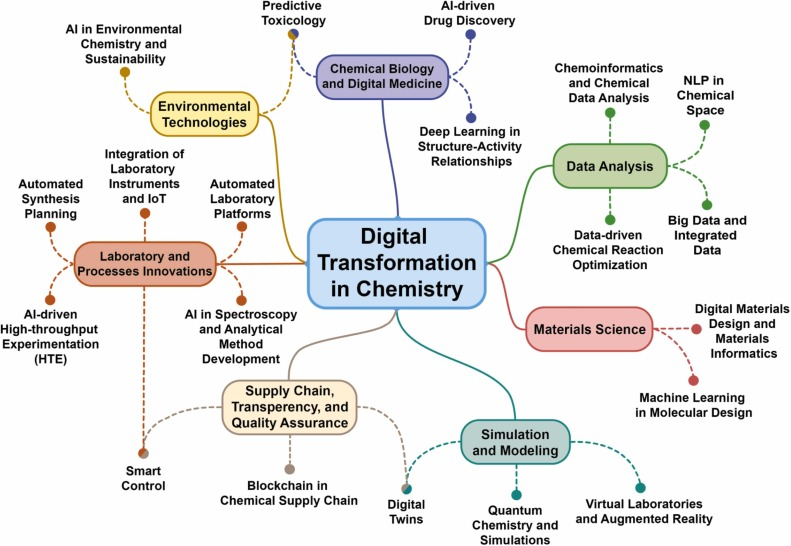
\includegraphics[width=0.7\textwidth]{images/digital_transformation_in_chemistry.jpg}
			\caption[pt9]{Связь технологий на основе ИИ с более широкими темами в зависимости от их применения.}
			\label{fig: digital_transformation_in_chemistry}
		\end{figure} 
	\end{frame}
	
	\begin{frame}{Формулировка проблемы}

	\begin{figure}[!tbp]
		\begin{subfigure}[b]{0.4\textwidth}
		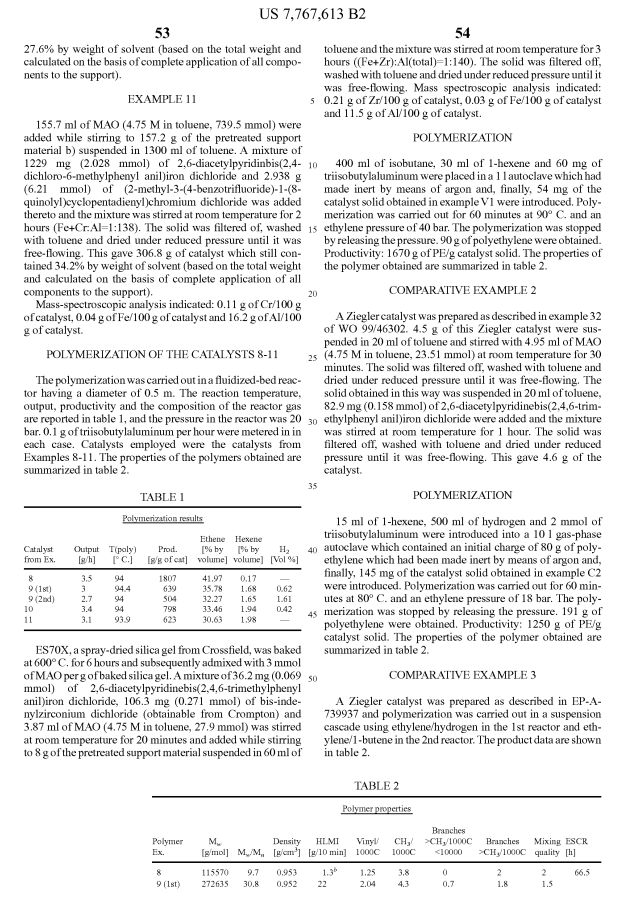
\includegraphics[width=1\textwidth]{images/patent_data_example.png}
			\caption{}
			\label{fig:patent_data_example}
		\end{subfigure}
		\hfill
		\begin{subfigure}[b]{0.4\textwidth}
		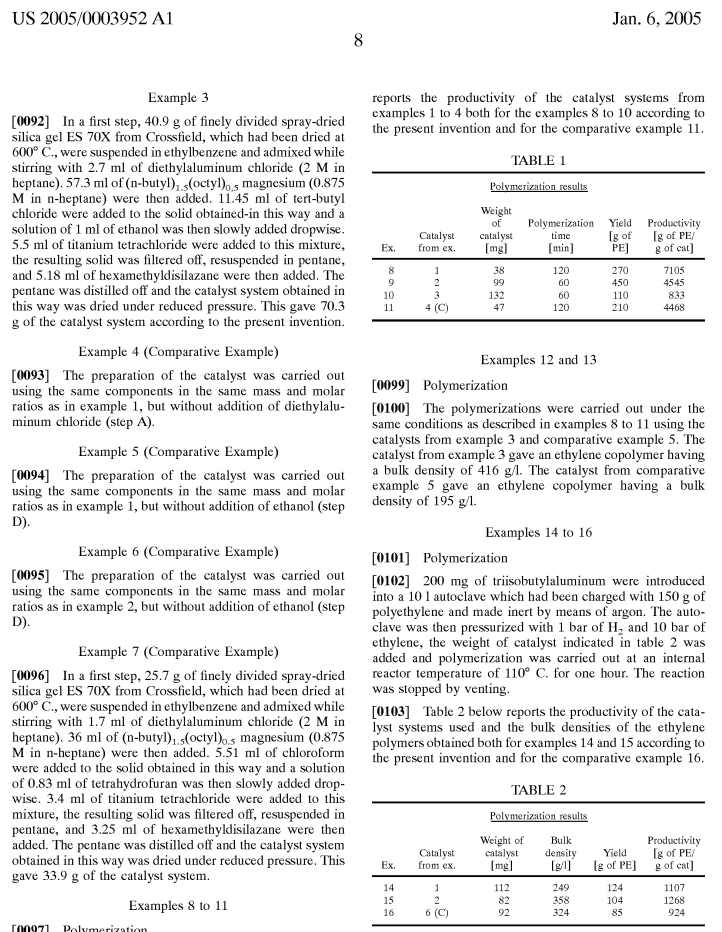
\includegraphics[width=1\linewidth]{images/patent_data_example_2}
			\caption{}
			\label{fig:patent_data_example_2}
		\end{subfigure}
		\caption{Примеры входных данных}
	\end{figure}

	\end{frame}

	\begin{frame}{Цели и задачи}

	 	\textbf{Цель работы:} Создать цифрового <<ассистента>> на основе большой языковой модели для извлечения структурированных данных из патентной документации\\~\
	 	\begin{outline}

	 	 Задачи:
	 		\1 Выбрать домен для проведения исследования и провести релевантный патентный поиск и создать БД документов для дальнейшего извлечения информации
	 		\1 Провести обзор современных фреймворков и технологий для работы с БЯМ 
	 		\1 Создать агентов на основе БЯМ способных решать следующие задачи:
	 		\2 Сегментация и фильтрация текста
	 		\2 Классификация текста и выделение информации о синтетических процедурах
	 		\2 Запрос к БЯМ
	 		\2 Формирование датасета
 		\end{outline}
	\end{frame}
	
	\begin{frame}{Обзор литературы}
		{\scriptsize2. Ramos M.C., Collison C.J., White A.D. A Review of Large Language Models and Autonomous Agents in Chemistry: arXiv:2407.01603. arXiv, 2024.}
		
		\begin{figure}
			\centering
			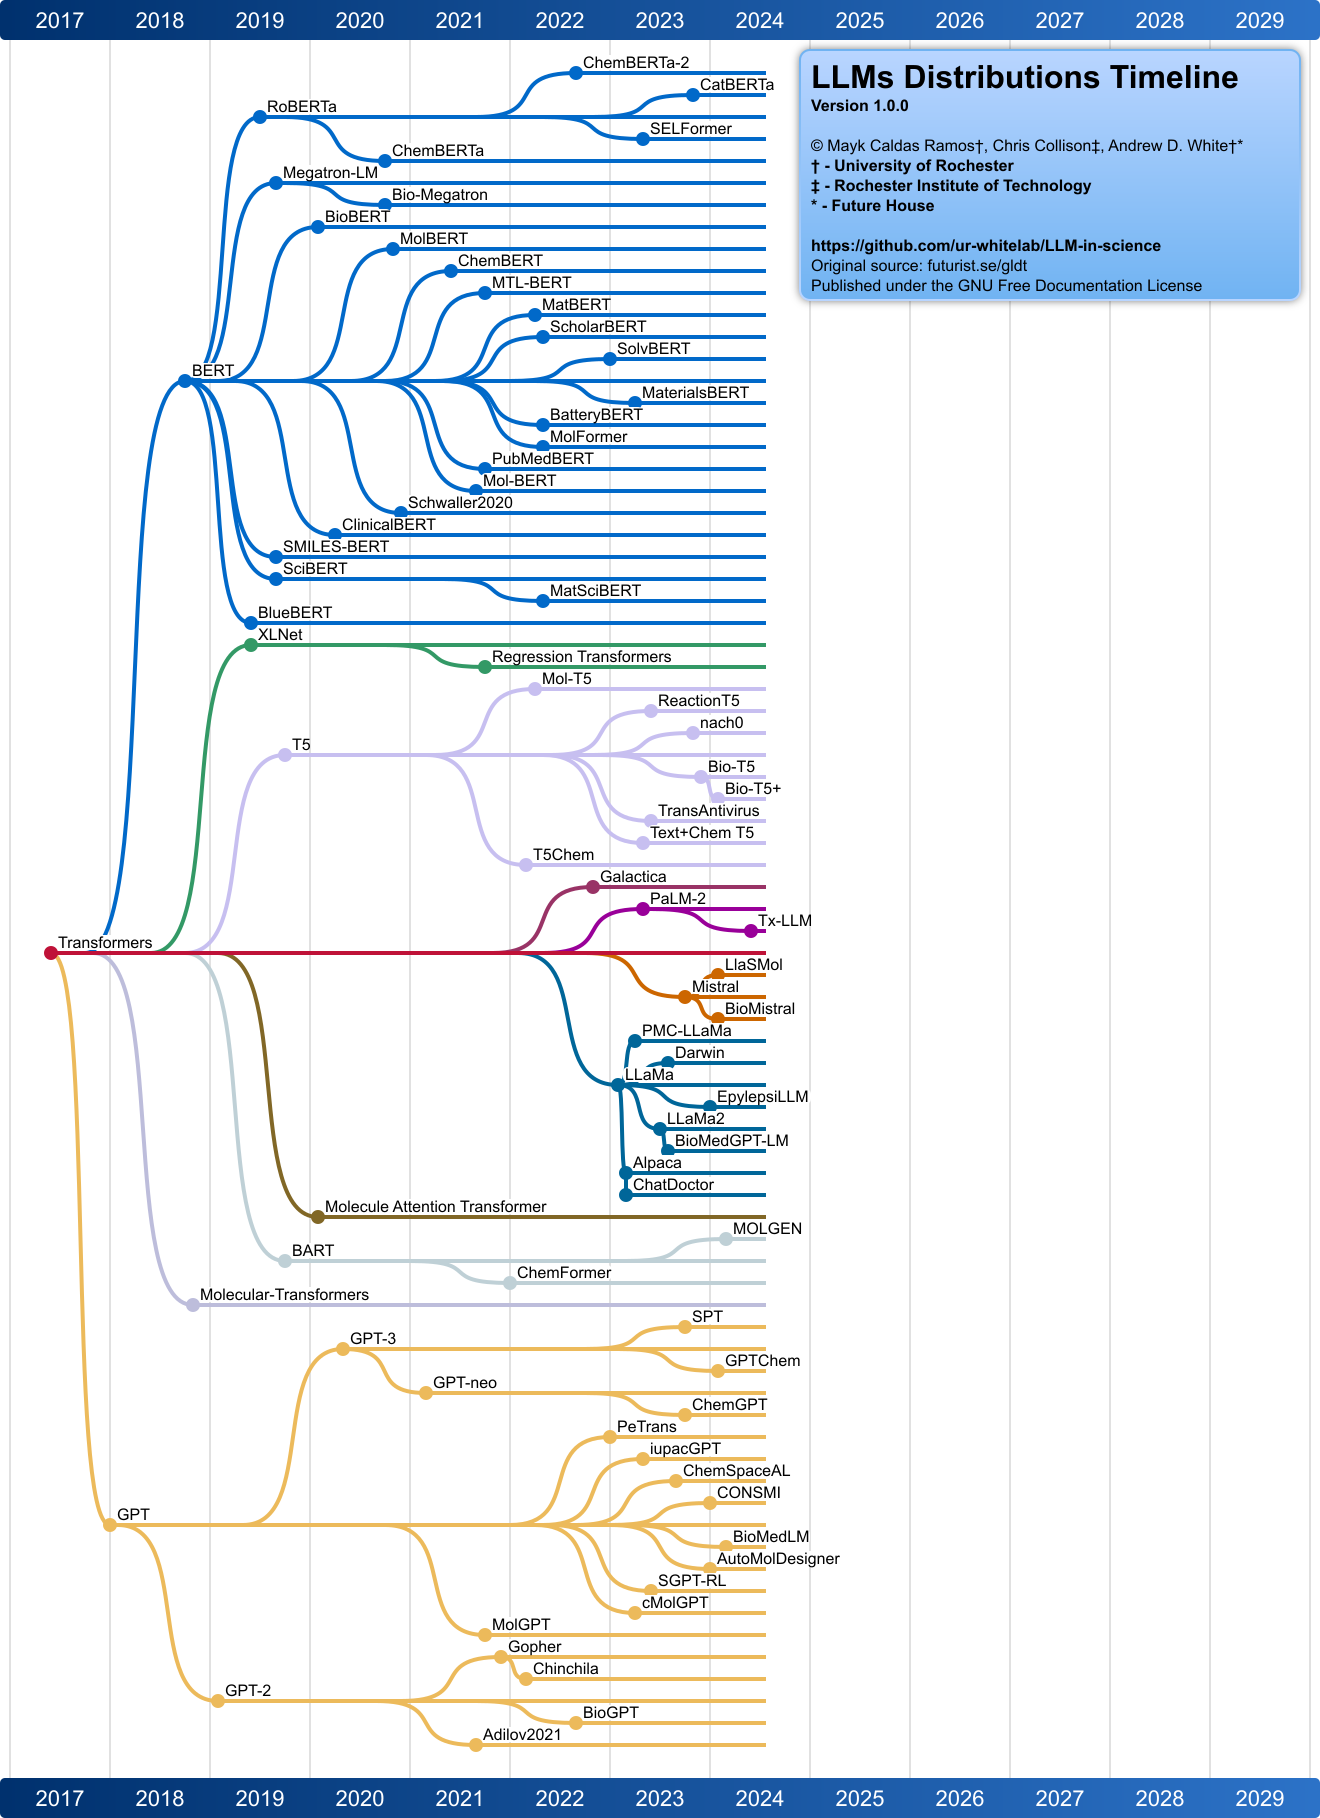
\includegraphics[width=0.58\textwidth, angle=90]{images/llm_ldt.png}
			\caption[pt9]{Иллюстрация хронологической эволюции больших языковых моделей.}
			\label{fig: llm_ldt}
		\end{figure}
		

	\end{frame}
	
	\begin{frame}{Обзор литературы}
		{\scriptsize 3. Lála J. et al. PaperQA: Retrieval-Augmented Generative Agent for Scientific Research: arXiv:2312.07559. arXiv, 2023.}
		\begin{figure}
	
	
	\centering
	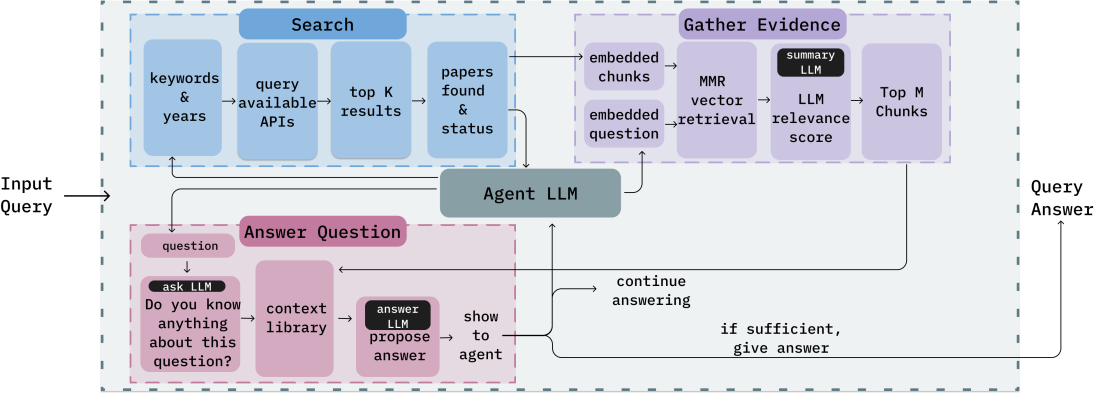
\includegraphics[width=1\textwidth]{images/PaperQA_Workflow_Diagram}
	\caption{PaperQA — это агент, который преобразует вопрос в ответ с указанием источников. Агент использует три инструмента: поиск, сбор данных и ответ на вопрос. Инструменты позволяют ему находить и анализировать соответствующие полнотекстовые исследовательские работы, определять конкретные разделы в работе, которые помогают ответить на вопрос, суммировать эти разделы с контекстом вопроса (называемые доказательствами), а затем генерировать ответ на основе доказательств.}
	\label{fig:paperqaworkflowdiagram}
		\end{figure}
		
		
	\end{frame}
	
	\begin{frame}{Обзор литературы}
		{\scriptsize4. Zheng Z. et al. ChatGPT Chemistry Assistant for Text Mining and Prediction of MOF Synthesis.}
		
\begin{figure}
	\centering
	\includegraphics[width=0.7\linewidth]{"images/Schematics of the ChatGPT Chemistry Assistant workflow"}
	\caption{ChatGPT Chemistry Assistant ChatGPT и ChemPrompt для эффективного анализа текста и обобщения условий синтеза MOF из разнообразного набора опубликованных исследовательских статей. }
	\label{fig:schematics-of-the-chatgpt-chemistry-assistant-workflow}
\end{figure}
	\end{frame}
	
	\begin{frame}{Текущие результаты и планы}

	\begin{table}\hspace*{-12pt}
	\begin{tabular}{cclllllllllllll}
		\rowcolor[HTML]{92D050} 
		\multicolumn{1}{l}{\cellcolor[HTML]{92D050}{\color[HTML]{FFFFFF} \textbf{Catalyst type:}}} &
		\multicolumn{11}{l}{\cellcolor[HTML]{92D050}{\color[HTML]{FFFFFF} \textbf{PE: ZN on SiO2}}} &
		&
		&
		\\
		\rowcolor[HTML]{EDEDED} 
		\textbf{KEY WORDS:} &
		\multicolumn{14}{c}{\cellcolor[HTML]{EDEDED}\textbf{\begin{tabular}[c]{@{}c@{}}T/A/C/D: (((((Ziegler-Natta catalyst+) or \\ (silica?supported Ziegler-Natta catalyst+)) \\ and (titanium +chloride)) and gas-phase) \\ and (PE or polyethylene))\end{tabular}}} \\
		\rowcolor[HTML]{EDEDED} 
		\textbf{RESTRICTION:}                            & \multicolumn{14}{c}{\cellcolor[HTML]{EDEDED}\textbf{ALL}}                                                  \\
		\rowcolor[HTML]{EDEDED} 
		{\color[HTML]{385724} \textbf{\begin{tabular}[c]{@{}c@{}}number of documents \\ before relevance \\ is determined\end{tabular}}} &
		\multicolumn{14}{c}{\cellcolor[HTML]{EDEDED}{\color[HTML]{385724} \textbf{There were about 2491 documents (ORBIT)}}} \\
		\rowcolor[HTML]{EDEDED} 
		{\color[HTML]{385724} \textbf{DATE}}             & \multicolumn{14}{c}{\cellcolor[HTML]{EDEDED}{\color[HTML]{385724} \textbf{Priority date from 01/01/2002}}} \\
		\rowcolor[HTML]{EDEDED} 
		{\color[HTML]{385724} \textbf{Date of research}} & \multicolumn{14}{c}{\cellcolor[HTML]{EDEDED}{\color[HTML]{385724} \textbf{13.03.2022}}}                    \\
		\rowcolor[HTML]{F2F2F2} 
		{\color[HTML]{1565C0} 2491}                      & \multicolumn{14}{c}{\cellcolor[HTML]{F2F2F2}{\color[HTML]{444444} patented inventions}}                    \\
		0,5                                              & \multicolumn{14}{c}{\cellcolor[HTML]{F2F2F2}{\color[HTML]{444444} owned by top 10 players}}               
	\end{tabular}
	\caption{результаты поиска по ключевым словам}
	\label{tab:  tab1 }
	\end{table}

		
	\end{frame}
	
	\begin{frame}{Текущие результаты и планы}
		
	\begin{figure}
		\centering
		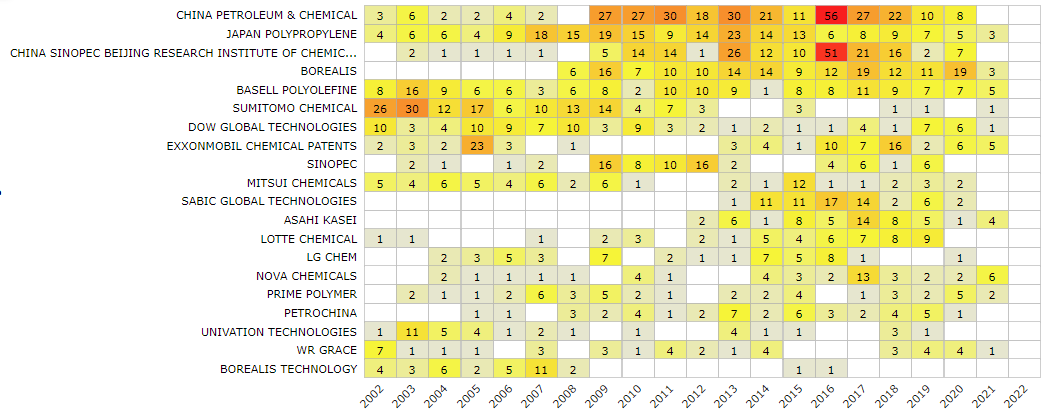
\includegraphics[width=1\linewidth]{images/patent_data_heatmap}
		\caption{Тепловая карта распределения патентов}
		\label{fig:patentdataheatmap}
	\end{figure}
		\end{frame}

\begin{frame}{Текущие результаты и планы}
	
	\textbf{План работ на третий семестр}\\
	\begin{outline} 
		\1 Создать набор агентов и инструментов для решения задачи извлечения информации на базе одной БЯМ (ChatGPT-3.5Turbo)
		\1 Собрать небольшой датасет (около 50-100 наблюдений) для оценки эффективности извлечения данных 
		\1 Оценить эффективность обработки данных с помощью метрики F1-score
	\end{outline}
\end{frame}
	\begin{frame}{Список литературы}

			1. Ananikov V. Top 20 Influential AI-Based Technologies in Chemistry. Chemistry, 2024.\\\medskip
			2. Ramos M.C., Collison C.J., White A.D. A Review of Large Language Models and Autonomous Agents in Chemistry: arXiv:2407.01603. arXiv, 2024.\\\medskip
			3. Lála J. et al. PaperQA: Retrieval-Augmented Generative Agent for Scientific Research: arXiv:2312.07559. arXiv, 2023.\\\medskip
			4. Zheng Z. et al. ChatGPT Chemistry Assistant for Text Mining and Prediction of MOF Synthesis.
	
	
	\end{frame}
\begin{frame}
\end{frame}
	
\end{document}


